\ifdefined\AINATemplate
\documentclass{svproc}
\providecommand{\orcidID}[1]{}
\else
\documentclass[runningheads]{llncs}
\fi
\usepackage[T1]{fontenc}
\usepackage{graphicx,amsmath,amssymb,booktabs}
\usepackage{url}
\usepackage[hidelinks]{hyperref}
\urlstyle{rm}
\newcommand{\KAcc}{87.5\%}
\newcommand{\KFone}{87.4\%}
\newcommand{\KPGDAcc}{0.03\%}
\newcommand{\KPGDTPR}{1.12\%}
\newcommand{\KPGDFPR}{4.97\%}
\newcommand{\KFedAcc}{48.0\%}
\newcommand{\SAcc}{86.0\%}
\newcommand{\SFone}{86.0\%}
\newcommand{\SPGDAcc}{0.46\%}
\newcommand{\SPGDTPR}{0.09\%}
\newcommand{\SPGDFPR}{6.85\%}
\newcommand{\SFedAcc}{46.3\%}
\newcommand{\KSourceAcc}{71.8\%}
\newcommand{\KSourcePGDAcc}{0.95\%}
\newcommand{\KSourceFPR}{7.3\%}


\begin{document}
\ifdefined\AINATemplate\mainmatter\fi
\title{SeF-MedFusion-Uproot: Reproducible Robustness Monitoring and Semantic Provenance for Histology and Cytology}
\titlerunning{Reproducible Robustness Monitoring and Semantic Provenance}
\author{Diogen Babuc\orcidID{0009-0000-5126-6480} \and Teodor-Florin Forti\c{s}\orcidID{0000-0002-3143-8908}}
\authorrunning{D. Babuc and T.-F. Forti\c{s}}
\institute{Faculty of Informatics, West University of Timi\c{s}oara, Romania\\
\email{\{diogen.babuc,florin.fortis\}@uvt.ro}}
\maketitle

\begin{abstract}
Auditable image predictions require reliability signals and a record of their origin. SeF-MedFusion-Uproot combines compact image classification with gradient--confidence monitoring and semantic provenance. A training-only parameter--gradient heuristic selects a network from a declared candidate pool. A detector combines pseudo-label input gradients with predictive uncertainty and uses clean held-out calibration. Predictions, input hashes, model hashes, and review flags are exported as RDF and checked using SHACL. Experiments use public Kather 2016 colorectal and SIPaKMeD cervical-cell images with three initialization seeds. Selected-model clean accuracies are \KAcc{} and \SAcc{}, respectively. PGD tests at $8/255$ yield successful-attack detection rates of \KPGDTPR{} and \SPGDTPR{}. Detector-aware attacks and a small federated aggregation simulation further delimit the evidence. Clinical staging is preserved only when externally supplied; no TNM stage is inferred from image classes.
\ifdefined\AINATemplate
\keywords{histopathology, cytology, adversarial detection, RDF provenance}
\else
\keywords{histopathology \and cytology \and adversarial detection \and semantic provenance \and reproducibility}
\fi
\end{abstract}

\section{Introduction}
Histological and cytological classifiers can attach a probability vector to an image without recording the model version, preprocessing, calibration rule, or source of the result. These omissions complicate auditing when predictions are exchanged between services or institutions. High confidence also provides no general protection against adversarially chosen inputs: small perturbations can change a prediction while retaining substantial confidence~\cite{goodfellow2015,madry2018}. A monitoring system therefore needs both measurable reliability signals and a record of how those signals were produced.

SeF-MedFusion-Uproot addresses this operational problem by coupling image inference with a lightweight detector and an explicit provenance graph. Its central output is an auditable prediction record: the image source, actual model input, checkpoint, confidence, gradient signal, detector configuration, and review flag can be connected without treating any one signal as a clinical decision. RDF provenance follows PROV-O~\cite{prov2013}; machine-checkable output constraints use SHACL~\cite{shacl2017}. This combination is useful for distributed information systems because each producer can emit the same record structure even when image processing remains local.

The contribution is an executable and deliberately bounded instantiation of this design. First, we specify the architecture pool, proxy direction, training procedure, and clean-data detector calibration. Second, we evaluate classification and attack detection separately on two public image datasets, including baselines that use only uncertainty, entropy, or gradients. Third, we validate graph constraints and query results against the original prediction events. A three-client, single-process FedAvg experiment additionally checks whether the selected network can be aggregated~\cite{mcmahan2017}. This simulation does not establish privacy or clinical interoperability.

The scope is patch and cell classification. Whole-slide multiple-instance learning, clinical diagnosis, and cancer staging are separate tasks. In particular, local tissue appearance does not supply the tumor extent, nodal involvement, and distant-metastasis evidence required by TNM~\cite{nci2025}. The implementation consequently records absent staging as unavailable and accepts externally supplied staging only with a source and staging-system metadata.

\section{Related Work and Evaluation Scope}
The Kather dataset introduced an eight-class colorectal texture benchmark~\cite{kather2016,katherdata2016}; SIPaKMeD provides isolated cervical cells derived from larger cluster images~\cite{plissiti2018}. These tasks differ from whole-slide prediction. Attention-based multiple-instance learning aggregates sets of instances into bag-level predictions~\cite{ilse2018}; CLAM extends this setting with clustering constraints~\cite{lu2021}. Applying their published numbers to independent patch or cell experiments would conflate different targets and evaluation protocols. We instead train all networks in a common, explicitly specified pool on identical partitions.

AD-ZeroNAS explores activation-diversity proxies for histopathological architecture search~\cite{babuc2025}. Here we evaluate a simpler parameter-to-gradient heuristic with a declared minimization direction. The pool contains three compact CNNs, enabling direct inspection of the relationship between the heuristic, network size, and measured prediction quality. This experiment does not reproduce the full AD-ZeroNAS search space or establish that the heuristic predicts general architecture rankings.

FGSM and projected gradient descent provide standard first-order adversarial stress tests~\cite{goodfellow2015,madry2018}. A detector must additionally be assessed against an adversary aware of its decision rule: evaluation against an unaware attack alone can overstate security~\cite{carlini2017}. We include a differentiable detector-aware objective, report its limitations, and retain false-positive rates on clean test images. The semantic layer complements these tests by preserving their provenance. Constraint conformance indicates well-formed records, rather than evidence that the predicted tissue label or any clinical interpretation is correct.

\section{Framework and Methods}
\subsection{Pipeline and Candidate Networks}
Figure~\ref{fig:architecture} summarizes the implemented pipeline. RGB inputs are resized to $64\times64$ using bilinear interpolation and scaled to $[0,1]$. No stain normalization or pretrained weights are used. Training augmentation consists of independently sampled horizontal and vertical flips and rotations by multiples of $90^{\circ}$. Tuning, calibration, and test images receive only the deterministic preprocessing.

\begin{figure}[t]
\centering
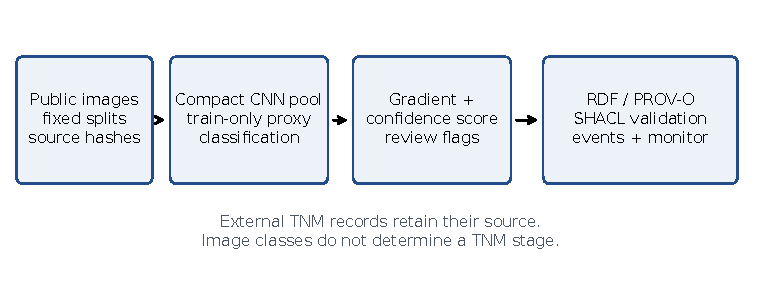
\includegraphics[width=\textwidth]{figures/architecture.pdf}
\caption{Implemented pipeline. The same model and calibration metadata are used for numerical evaluation, provenance export, and the local event monitor.}
\label{fig:architecture}
\end{figure}

Each candidate has three blocks with output channels $(w,2w,4w)$, where $w\in\{8,16,32\}$. Every block contains two bias-free $3\times3$ convolutions, each followed by four-group normalization and ReLU, and ends with $2\times2$ max pooling. Global average pooling and a linear layer produce class logits. Group normalization avoids coupling one image's inference-time gradient to other images in a minibatch. The implementation tests this property by comparing signals computed individually and in batches.

For architecture $a$, the selection heuristic is
\begin{equation}
 Q(a)=\frac{P_a}{\max\{B^{-1}\sum_{b=1}^{B}\|\nabla_{\theta_a}\mathcal{L}_b\|_2,\eta\}},
 \qquad a^*=\arg\min_a Q(a),
 \label{eq:proxy}
\end{equation}
where $P_a$ is the trainable parameter count, $B=3$ training minibatches of 64 images are shared across candidates, $\mathcal{L}_b$ is mean cross-entropy using their training labels, and $\eta=10^{-12}$ guards division. The norm combines all parameter gradients. The candidates are randomly initialized with the declared seed; no tuning, calibration, test, or attacked image is used for proxy computation. The numerator favors compact models, while, at fixed size, minimizing $Q$ rewards larger gradient norms. Neither effect establishes training stability or adversarial robustness.

For auditability, every candidate is also trained from a fresh initialization under the same protocol. These additional runs evaluate the pool; they are not required by proxy-based deployment. Proxy computation does not change the eventual training initialization or consume its random sequence. The final checkpoint for each candidate is the epoch with highest tuning macro F1, with the earliest epoch retained on ties.

\subsection{Gradient--Confidence Monitoring}
The detector operates without ground-truth labels at inference. Let $p_k(x)$ be the softmax probability and $\tilde y(x)=\arg\max_k p_k(x)$ a detached pseudo-label. Define
\begin{align}
 g(x)&=\left\|\nabla_x\left[-\log p_{\tilde y(x)}(x)\right]\right\|_2,\\
 u(x)&=1-\max_k p_k(x),\\
 d(x)&=\alpha\min\{g(x)/s_g,1\}+(1-\alpha)u(x),\quad \alpha=0.5,
 \label{eq:detector}
\end{align}
where $s_g=\max_{x\in D_{\mathrm{cal}}}g(x)$ is fitted once on the clean calibration partition. The denominator is bounded below by $10^{-12}$. It is never recomputed from a test batch. Clipping keeps $d(x)\in[0,1]$ when a future gradient exceeds its calibration range.

The review threshold is the empirical 95th percentile of clean calibration scores, using the higher-order-statistic convention. A sample is flagged precisely when $d(x)>\tau$. This choice targets a nominal 5\% calibration alarm rate; it does not force the test false-positive rate to 5\%. We separately calibrate analogous thresholds for $u(x)$, normalized $g(x)$, and entropy $h(x)=-\sum_k p_k(x)\log p_k(x)$. No adversarial images or test labels are used to fit these detectors.

Input gradients are obtained from a sum of per-image losses, so their scale does not change with batch size. A detector flag requests review and does not identify the cause of an unusual input. The method neither repairs perturbed images nor changes the classifier's prediction. Detection therefore cannot, by itself, raise adversarial classification accuracy.

\subsection{Provenance, Constraints, and Monitoring}
Samples, models, predictions, processing runs, and datasets are represented in a local vocabulary that also covers external TNM records. Prediction entities reference the processed input, checkpoint, predicted class, confidence, gradient norm, combined score, review flag, and generating activity. SHA-256 identifiers distinguish the original image file, the resized floating-point model input, and the saved checkpoint. Perturbed inputs receive their own hashes and remain linked to the original source. Run metadata stores the configuration and seed. The vocabulary uses a proposed research namespace and is not presented as an established clinical ontology.

PROV-O links express generation, derivation, and resource use~\cite{prov2013}. SHACL shapes enforce cardinalities, numeric domains, required sample and model links, and stage-status consistency~\cite{shacl2017}. Confidence and combined scores must lie in $[0,1]$; gradient norms must be nonnegative. An externally supplied TNM record requires separate T, N, and M strings, staging system, edition, and source IRI. No staging rules are applied to predicted image classes, and neither experimental dataset supplies TNM labels for evaluation.

The exported event stream and RDF graph describe the same predictions. A SPARQL count of flagged prediction entities is checked against a direct event count. Validation also includes negative controls, such as an out-of-range confidence or a missing model link. The local monitor reads JSONL events and exposes prediction volume, mean confidence, and review flags. It runs on the loopback interface and refreshes every two seconds. This is an operational prototype; it includes no clinical workflow integration, authentication service, or certified alerting guarantee.

\section{Experimental Protocol}
\subsection{Data and Partitions}
\begin{table}[t]
\centering
\caption{Dataset partitions after duplicate removal. SIPaKMeD is split by source cluster; Kather is split at tile level.}
\label{tab:data}
\small
\setlength{\tabcolsep}{4pt}
\begin{tabular}{lrrrrr}
\toprule
Dataset & Classes & Train & Tune & Calib. & Test \\
\midrule
Kather 2016 & 8 & 3000 & 504 & 496 & 1000 \\
SIPaKMeD & 5 & 2318 & 479 & 391 & 861 \\
\bottomrule
\end{tabular}
\end{table}

Kather 2016 contains 5,000 $150\times150$ RGB colorectal tissue tiles, with 625 tiles in each of eight classes~\cite{kather2016,katherdata2016}. Its categories include tumor epithelium, simple and complex stroma, immune cells, debris, mucosal glands, adipose tissue, and background. We split available tiles by class into approximately 60\% training, 10\% tuning, 10\% calibration, and 20\% test data. Tile names do not provide a validated patient grouping for this experiment. This is consequently a tile-level internal evaluation, which may retain slide-related dependencies; it cannot support patient-level or external-center generalization claims.

SIPaKMeD contains 4,049 isolated cells from 966 source cluster images and five cell categories: superficial/intermediate, parabasal, koilocytotic, metaplastic, and dyskeratotic~\cite{plissiti2018}. We use the cropped RGB cell images and derive a source-group key from the official class directory and cluster identifier in each filename. All cells from a source cluster stay in one partition. Groups are shuffled within each class and assigned in the same approximate 60/10/10/20 proportions. Group sizes vary, so image-level counts differ from these proportions. The available grouping is at cluster-image level, not a demonstrated patient-level split.

The split seed is 2027 and is fixed across training seeds. Exact source-pixel duplicates are removed before partitioning, and the resulting manifest records every retained filename, class, group, split, and hash. Table~\ref{tab:data} reports the actual retained counts. Source archive checksums and download locations are also recorded. The cervical targets are cell categories rather than ASC/LSIL/HSIL diagnostic labels; neither dataset supplies TNM outcome labels.

\subsection{Training and Stress Tests}
Each network is trained for 25 epochs with AdamW, learning rate $10^{-3}$, weight decay $10^{-4}$, batch size 64, and cosine learning-rate decay. Initialization seeds are 17, 29, and 41. The tuning set selects an epoch; the disjoint calibration set fits detector normalization and thresholds. Test data are used only for the reported evaluation. Mean and sample standard deviation across the three initialization seeds describe optimization variability on one fixed partition, rather than independent patient cohorts.

We apply untargeted FGSM and random-start PGD with $\ell_{\infty}$ budgets $\epsilon\in\{4/255,8/255\}$ to all test images. PGD uses 20 steps, step size $2/255$, and one uniform random start. Projection enforces both the perturbation box and valid $[0,1]$ pixels. Attacks use true labels to maximize cross-entropy. Gaussian noise with standard deviation $8/255$, followed by clipping, is a separate corruption condition; it is not constrained by the adversarial $\ell_{\infty}$ budget.

The detector-aware test maximizes
\begin{equation}
 \mathcal{J}(x')=\mathcal{L}(x',y)-\lambda d(x'),\qquad\lambda=1,
 \label{eq:adaptive}
\end{equation}
using 20 projected steps and $\epsilon=8/255$. It differentiates through the input-gradient norm, retaining second-order derivatives while treating the current pseudo-label as fixed in each step. To bound computation, it uses 128 initially correct test images sampled with a declared seed. The same clean subset provides its reference false-positive rate. A single objective weight, start, and attack length do not establish robustness to an optimal adaptive adversary~\cite{carlini2017}.

Classification metrics include accuracy, macro F1 over all dataset classes, negative log-likelihood, Brier score, and 15-bin expected calibration error (ECE). Attack success rate (ASR) counts newly incorrect predictions among initially correct images. Detector AUROC compares all evaluated perturbed images with their clean counterparts. We report both the detection rate on all perturbed inputs in the artifact and the successful-attack detection rate (TPR$_s$) in the paper, together with clean false-positive rate (FPR). These denominators are kept distinct.

Experiments run with CPU PyTorch, deterministic algorithms, and four worker threads on a Windows x86-64 machine with an AMD processor exposing 16 logical CPUs. Checkpoints, per-image predictions, raw detector signals, and metric records are saved. Single-image forward and forward-plus-detector timings use five warmups and 30 repetitions. They exclude image loading, resizing, graph serialization, and user-interface refresh. Graph construction and complete-graph SHACL validation are measured separately.

\section{Results and Discussion}
\subsection{Classification and Selection}
\begin{table}[t]
\centering
\caption{Clean test performance (percent, mean $\pm$ sample SD over three initialization seeds). Width denotes the first block channel count; * marks proxy selection. ECE uses 15 bins.}
\label{tab:classification}
\small
\setlength{\tabcolsep}{4pt}
\begin{tabular}{llrrrr}
\toprule
Dataset & Width & Params (k) & Accuracy & Macro F1 & ECE \\
\midrule
Kather 2016 & 8* & 18.6 & 87.5 $\pm$ 1.7 & 87.4 $\pm$ 1.7 & 3.7 $\pm$ 0.5 \\
Kather 2016 & 16 & 72.8 & 88.2 $\pm$ 0.2 & 88.1 $\pm$ 0.2 & 2.9 $\pm$ 0.2 \\
Kather 2016 & 32 & 288.5 & 88.3 $\pm$ 1.5 & 88.3 $\pm$ 1.4 & 2.7 $\pm$ 0.5 \\
SIPaKMeD & 8* & 18.5 & 86.0 $\pm$ 1.8 & 86.0 $\pm$ 1.7 & 3.9 $\pm$ 1.1 \\
SIPaKMeD & 16 & 72.6 & 86.5 $\pm$ 2.9 & 86.4 $\pm$ 2.9 & 3.3 $\pm$ 0.8 \\
SIPaKMeD & 32 & 288.1 & 87.0 $\pm$ 1.7 & 86.8 $\pm$ 1.7 & 3.2 $\pm$ 0.4 \\
\bottomrule
\end{tabular}
\end{table}

The proxy-selected networks achieve mean clean accuracies of \KAcc{} on Kather and \SAcc{} on SIPaKMeD; their macro F1 scores are \KFone{} and \SFone{}. Table~\ref{tab:classification} reports every candidate under the same training and checkpoint-selection protocol. Parameter counts are measured from the implemented models rather than inferred from architecture names. Predictive confidence and calibration metrics are retained in the machine-readable results; a high confidence value is not used as a synonym for reliability.

The small candidate pool supports an audit of the implemented selection rule. It does not justify a general claim that zero-shot selection matches a broad architecture search or state-of-the-art whole-slide models. Furthermore, the cost of training all candidates in this study must not be mistaken for the deployment cost of training only the selected candidate. Tuning trajectories and per-run checkpoint choices are available in the artifact.

As a sensitivity analysis, we additionally hold out complete Kather filename families. Prefixes \texttt{CRC-Prim-HE-01} through \texttt{-10} are assigned to six training, one tuning, one calibration, and two test groups using seed 2027. A width-8 model is retrained with initialization seed 17 and the same optimizer protocol. It obtains \KSourceAcc{} clean accuracy and \KSourcePGDAcc{} under PGD-$8/255$, with \KSourceFPR{} clean FPR. The inferred families remain disjoint, but are not independently verified patient identifiers. Exact assignments and sample counts are included in the artifact; this single-seed analysis is separate from Table~\ref{tab:classification}.

\subsection{Attack Detection and Remaining Errors}
\begin{table}[t]
\centering
\caption{Selected-model stress tests (percent, mean $\pm$ SD). Budgets are in units of $1/255$. ASR counts new errors among initially correct images; TPR$_s$ is detection on those successful perturbations. Gaussian noise uses the indicated standard deviation. Adaptive uses 128 initially correct test images per seed.}
\label{tab:attacks}
\small
\setlength{\tabcolsep}{4pt}
\begin{tabular}{llrrr}
\toprule
Dataset & Condition & Accuracy & ASR & TPR$_s$ \\
\midrule
Kather 2016 & FGSM 4 & 27.73 $\pm$ 4.02 & 68.90 $\pm$ 5.54 & 20.38 $\pm$ 10.49 \\
Kather 2016 & FGSM 8 & 15.37 $\pm$ 2.03 & 82.80 $\pm$ 2.39 & 11.14 $\pm$ 2.82 \\
Kather 2016 & PGD 4 & 1.97 $\pm$ 1.50 & 97.73 $\pm$ 1.78 & 1.61 $\pm$ 0.82 \\
Kather 2016 & PGD 8 & 0.03 $\pm$ 0.06 & 99.96 $\pm$ 0.07 & 1.12 $\pm$ 1.56 \\
Kather 2016 & Noise 8 & 76.63 $\pm$ 6.25 & 14.79 $\pm$ 8.91 & 61.99 $\pm$ 38.67 \\
Kather 2016 & Adaptive 8 & 8.07 $\pm$ 13.98 & 91.93 $\pm$ 13.98 & 1.65 $\pm$ 1.29 \\
SIPaKMeD & FGSM 4 & 44.91 $\pm$ 6.48 & 47.68 $\pm$ 8.72 & 20.19 $\pm$ 7.93 \\
SIPaKMeD & FGSM 8 & 34.57 $\pm$ 5.00 & 60.00 $\pm$ 6.55 & 9.65 $\pm$ 6.62 \\
SIPaKMeD & PGD 4 & 9.68 $\pm$ 3.89 & 88.81 $\pm$ 4.35 & 0.91 $\pm$ 0.67 \\
SIPaKMeD & PGD 8 & 0.46 $\pm$ 0.40 & 99.46 $\pm$ 0.46 & 0.09 $\pm$ 0.08 \\
SIPaKMeD & Noise 8 & 72.94 $\pm$ 8.95 & 18.31 $\pm$ 10.06 & 49.13 $\pm$ 9.89 \\
SIPaKMeD & Adaptive 8 & 0.26 $\pm$ 0.45 & 99.74 $\pm$ 0.45 & 0.00 $\pm$ 0.00 \\
\bottomrule
\end{tabular}
\end{table}

PGD at $8/255$ leaves accuracies of \KPGDAcc{} on Kather and \SPGDAcc{} on SIPaKMeD. The combined monitor detects \KPGDTPR{} and \SPGDTPR{} of successful attacks, respectively, with clean test false-positive rates of \KPGDFPR{} and \SPGDFPR{}. These operating points use the declared clean calibration rule. Table~\ref{tab:attacks} also includes weaker budgets, corruption, and the detector-aware stress test.

\begin{table}[t]
\centering
\caption{Detector ablation on PGD-20 at $8/255$. Every threshold is independently calibrated on clean calibration data at the 95th percentile. AUROC uses all clean and perturbed test images; TPR$_s$ uses successful attacks.}
\label{tab:detectors}
\small
\setlength{\tabcolsep}{4pt}
\begin{tabular}{llrrr}
\toprule
Dataset & Detector & AUROC & TPR$_s$ (\%) & FPR (\%) \\
\midrule
Kather 2016 & 1 - confidence & 0.387 $\pm$ 0.064 & 0.84 $\pm$ 0.36 & 4.30 $\pm$ 0.66 \\
Kather 2016 & Entropy & 0.378 $\pm$ 0.060 & 1.03 $\pm$ 0.70 & 4.23 $\pm$ 0.81 \\
Kather 2016 & Gradient & 0.378 $\pm$ 0.088 & 2.14 $\pm$ 3.13 & 4.47 $\pm$ 0.32 \\
Kather 2016 & Combined & 0.380 $\pm$ 0.077 & 1.12 $\pm$ 1.56 & 4.97 $\pm$ 0.50 \\
SIPaKMeD & 1 - confidence & 0.335 $\pm$ 0.082 & 0.18 $\pm$ 0.21 & 4.84 $\pm$ 0.64 \\
SIPaKMeD & Entropy & 0.320 $\pm$ 0.084 & 0.13 $\pm$ 0.13 & 4.61 $\pm$ 0.60 \\
SIPaKMeD & Gradient & 0.319 $\pm$ 0.067 & 0.09 $\pm$ 0.08 & 7.28 $\pm$ 1.95 \\
SIPaKMeD & Combined & 0.326 $\pm$ 0.077 & 0.09 $\pm$ 0.08 & 6.85 $\pm$ 0.35 \\
\bottomrule
\end{tabular}
\end{table}

Table~\ref{tab:detectors} separates the contribution of each signal. The uncertainty and entropy baselines share the same trained classifier and receive independent clean calibration, making comparisons at the stated operating points interpretable. Figure~\ref{fig:roc} reports the threshold-free ROC behavior for the first seed. It is descriptive of that run; the table summarizes all three seeds. AUROC includes attacks that did not alter an initially correct prediction, whereas TPR$_s$ includes only successful attacks, so the metrics answer different questions.

\begin{figure}[t]
\centering
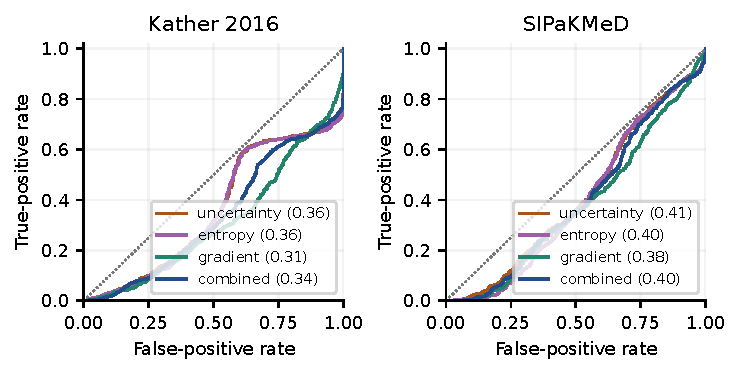
\includegraphics[width=\textwidth]{figures/roc.pdf}
\caption{Detector ROC curves for PGD-20 at $8/255$ using seed 17. Parenthesized legend values are AUROC. All test images are included in the clean/perturbed discrimination task.}
\label{fig:roc}
\end{figure}

On Kather 2016, mean PGD-$8/255$ AUROC is 0.380 for the combined score and 0.387 for the strongest single-signal baseline (uncertainty).

On SIPaKMeD, mean PGD-$8/255$ AUROC is 0.326 for the combined score and 0.335 for the strongest single-signal baseline (uncertainty).

In each dataset, the mean AUROC of the combined score is below 0.5. Its fixed score direction ranks attacked inputs poorly relative to clean images.

The combination does not provide a uniform AUROC improvement over the strongest single-signal baseline across these datasets. Its contribution must therefore be judged from the measured operating points rather than presumed from combining signals.

The adaptive condition uses a different, initially correct subset; its classification accuracy and detection rate should not be compared directly with whole-test-set PGD as if their denominators were identical.


\begin{figure}[t]
\centering
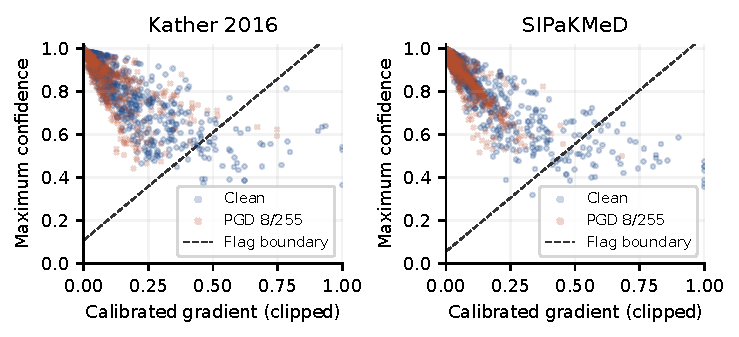
\includegraphics[width=\textwidth]{figures/signals.pdf}
\caption{Measured signals for clean and PGD-$8/255$ test images, seed 17. The dashed line is the calibrated combined-score boundary; points below it are flagged. The plot uses the fixed calibration normalizer rather than assuming separated clean and adversarial clusters.}
\label{fig:signals}
\end{figure}

Figure~\ref{fig:signals} connects the operating-point results to the observed signals. For a confident incorrect prediction, pseudo-label cross-entropy can be small and its gradient can also be small. Thus, an attack need not produce the high-gradient, low-confidence combination assumed by the review heuristic. Using a true-label loss instead would define a different signal that requires information unavailable during ordinary inference.

Detecting a proportion of successful perturbations does not make the unmodified classifier robust. Attacked images can remain misclassified, missed alarms can occur, and clean images can be flagged. Likewise, low-confidence natural errors and corrupted images can share the same signal patterns. The gradient--confidence score is therefore an auditable review heuristic. Claims of guaranteed adversarial identification, improved clinical safety, or a universal advantage over uncertainty alone are not supported by this protocol.

\subsection{System Checks and Federated Simulation}
\begin{table}[t]
\centering
\caption{Measured system checks for seed 17. Insert is graph construction time per prediction, SHACL is full-graph validation time, and monitor is median forward-plus-detector latency averaged across three seeds (batch size 1).}
\label{tab:systems}
\small
\setlength{\tabcolsep}{4pt}
\begin{tabular}{lrrrrr}
\toprule
Dataset & Pred. & Triples & Insert (ms) & SHACL (s) & Monitor (ms) \\
\midrule
Kather 2016 & 2000 & 36063 & 2.09 & 7.49 & 3.16 \\
SIPaKMeD & 1722 & 31059 & 2.18 & 5.84 & 3.39 \\
\bottomrule
\end{tabular}
\end{table}

For seed 17, the semantic evaluation exports each clean test prediction and its PGD-$8/255$ counterpart. The exported graphs conform to the declared shapes; injected invalid confidence values are rejected. SPARQL flag counts equal event-stream counts, and no TNM stages are inferred. Table~\ref{tab:systems} gives actual graph sizes and timings. These checks establish structural consistency and provenance recoverability, not clinical correctness or throughput under concurrent hospital workloads.

A separate FedAvg simulation uses the selected network, three balanced IID clients drawn only from training data, five communication rounds, and one local epoch per round. Models are averaged using local sample counts. The final-round test accuracies are \KFedAcc{} and \SFedAcc{}, respectively; full round trajectories are recorded. This is a functional experiment with a shorter optimization budget than centralized training. No non-IID institutions, secure aggregation, differential privacy, communication delays, or adversarial clients are simulated, and no privacy guarantee is claimed.

\section{Limitations and Reproducibility}
This study evaluates compact networks at reduced resolution, with one partition and three initialization seeds. The Kather split is not patient-disjoint, and SIPaKMeD grouping stops at the source cluster. Neither experiment measures prospective diagnostic performance, whole-slide analysis, external-site transfer, clinical staging accuracy, or an expert's interpretation of alerts. The semantic schema is deliberately small and has not undergone interoperability testing with a hospital information system or biomedical ontology alignment.

The adversarial evaluation uses one PGD start and a limited adaptive objective. Stronger attacks, alternative losses, multiple restarts, and attacks on acquisition or staining should be investigated before making security claims. Maximum-gradient calibration can be affected by calibration outliers, while clipping can discard distinctions above the fitted range. A nominal clean calibration quantile also provides no distribution-free guarantee for future alarm rates.

The accompanying artifact contains executable download and preprocessing code, exact split manifests, configuration, training histories, trained checkpoints, per-image outputs, detector calibration, RDF exports, event logs, unit tests, and scripts that regenerate paper tables and figures. A verification command recomputes metrics from saved arrays and checks checkpoint hashes, perturbation bounds, graph conformance, and query/event agreement. An additional training recheck independently repeats the selected first-seed run and compares weights and predictions. Large source datasets are downloaded from their original providers rather than redistributed with the repository.

\section{Conclusion}
SeF-MedFusion-Uproot provides an executable connection between image classification, gradient--confidence review signals, and provenance-aware monitoring. Its main practical contribution is that each reported result can be traced to a declared dataset partition, model checkpoint, detector calibration, and semantic record. The experiments expose differences between clean prediction quality, attack detection, and sensitivity to the data partition. Broader architecture search, stronger adaptive evaluation, external clinical data, and institution-level distributed testing remain necessary before extending these results to deployment claims.

\ifdefined\AINATemplate
\subsubsection*{Acknowledgments}
\else
\begin{credits}
\subsubsection{Acknowledgments}
\fi
This research was partially supported by the project ``Romanian Hub for Artificial Intelligence -- HRIA'', program \path{PCIDIF/709/PCIDIF_P4/OP1/RSO1.6/PCIDIF_A12}, Action 4.1, MySMIS 351416.
\ifdefined\AINATemplate\else\end{credits}\fi

\ifdefined\AINATemplate
\bibliographystyle{splncs03}
\else
\bibliographystyle{splncs04}
\fi
\bibliography{references}
\end{document}

